\subsection{Structure Preparation}\label{subsec:strucutre_prep}

In order to study the behavior of non-polar interaction in the solvation process, the free energy calculation, and how these two properties are related to the volume (size) of the molecules, a total of 20 structures were prepared to preform MD simulations using VMD-\texttt{molefacture} plugin \cite{humphrey1996vmd}. This tool has been designed to facilitate the construction and parameterisation of small molecules. It additionally provides a simple interface to prepare structures and files. These structures classifies as follows:
\begin{itemize}
    \item \underline{10 helix $n$-Alanines:} These correspond to the ``natural" configurations of the alanines with curvatures present on they structures. (Figure \ref{fig:5ALAhelix})
    \item \underline{10 extended $n$-Alanines:} They conformation where fixed to maintain a straight configuration along an axis. (Figure \ref{fig:5ALAext})
\end{itemize}   
with $n$ ranging from 1 ($ALA_1$)  to 10 ($ALA_{10}$) in both configurations. The peptide terminals where capped with with neutral amino-terminal ($NH_2$) and C-terminal ($COOH$). From this point, every step was preform using GROMOS molecular simulation software \cite{basharat2016structure}. 

\begin{figure}[h]
    \centering
    \begin{subfigure}[t]{0.45\textwidth}
    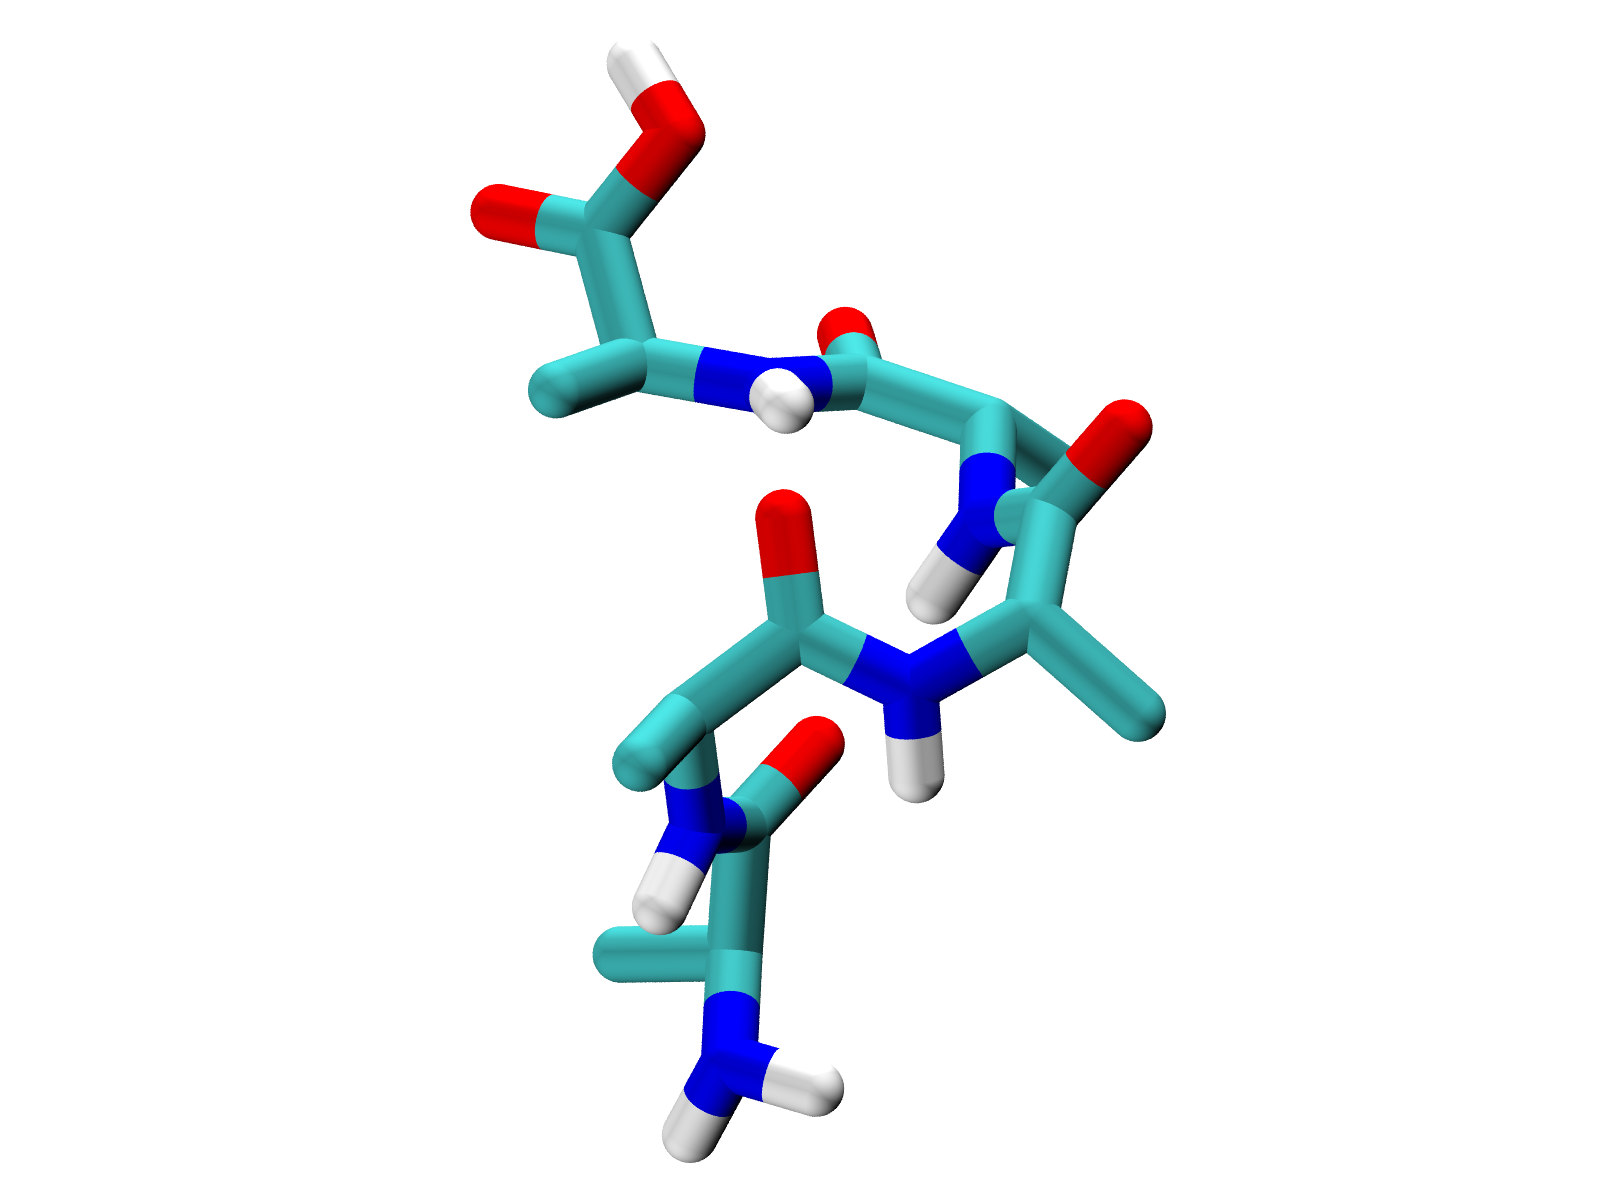
\includegraphics[width=\textwidth]{Figures/Chapter_5/5ALA_helix.png}
    \caption{Representation of helix-($ALA_5$) configuration.}
    \label{fig:5ALAhelix}
    \end{subfigure}
    \hspace{0.5cm}
    \begin{subfigure}[t]{0.45\textwidth}
    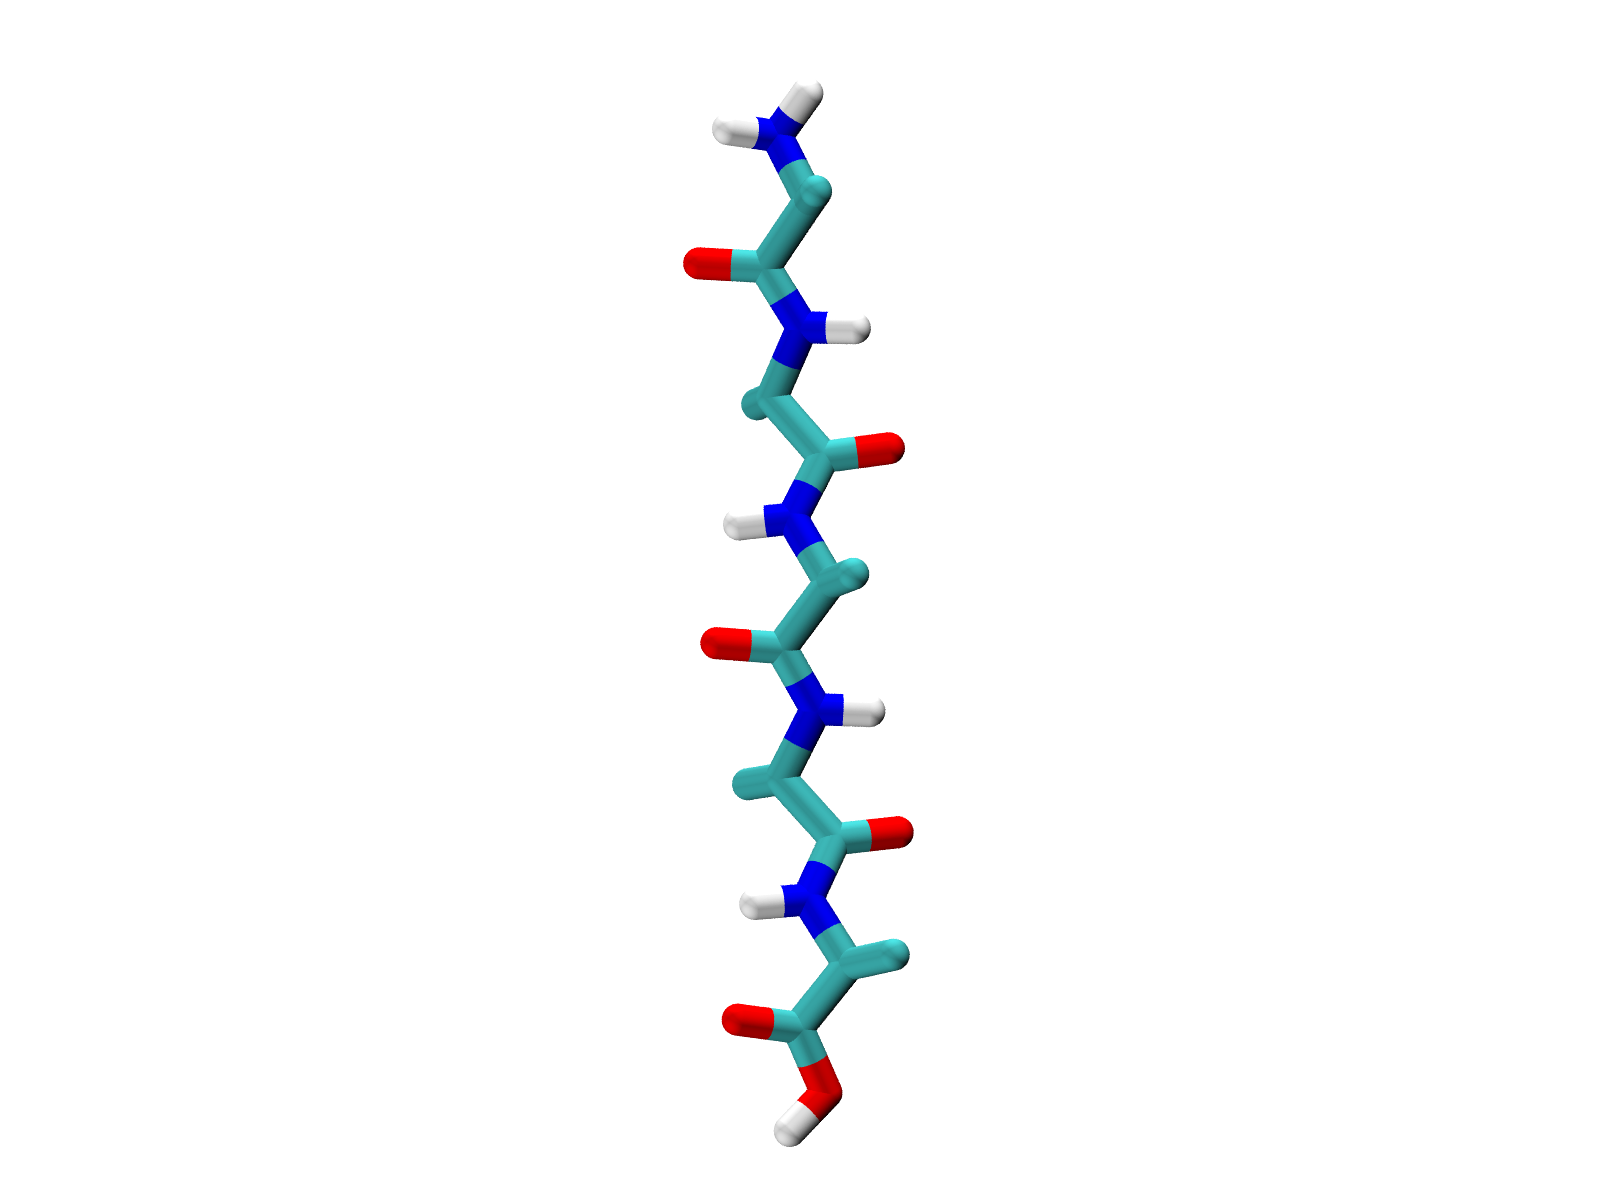
\includegraphics[width=\textwidth]{Figures/Chapter_5/5ALA_extended.png}
    \caption{Representation of extended-($ALA_5$) configuration.}
    \label{fig:5ALAext}
    \end{subfigure}
    
    \caption{Graphic representation of both penta-Alanines (helix and extended) configurations generated with VMD.}
    \label{fig:5_ALA_struct}
\end{figure}

